In this section we will make a custom gnuradio flow to perform a \gls{mitm} attack on our two feathers, as shown in \cref{mitm}.

\centrefigurestart
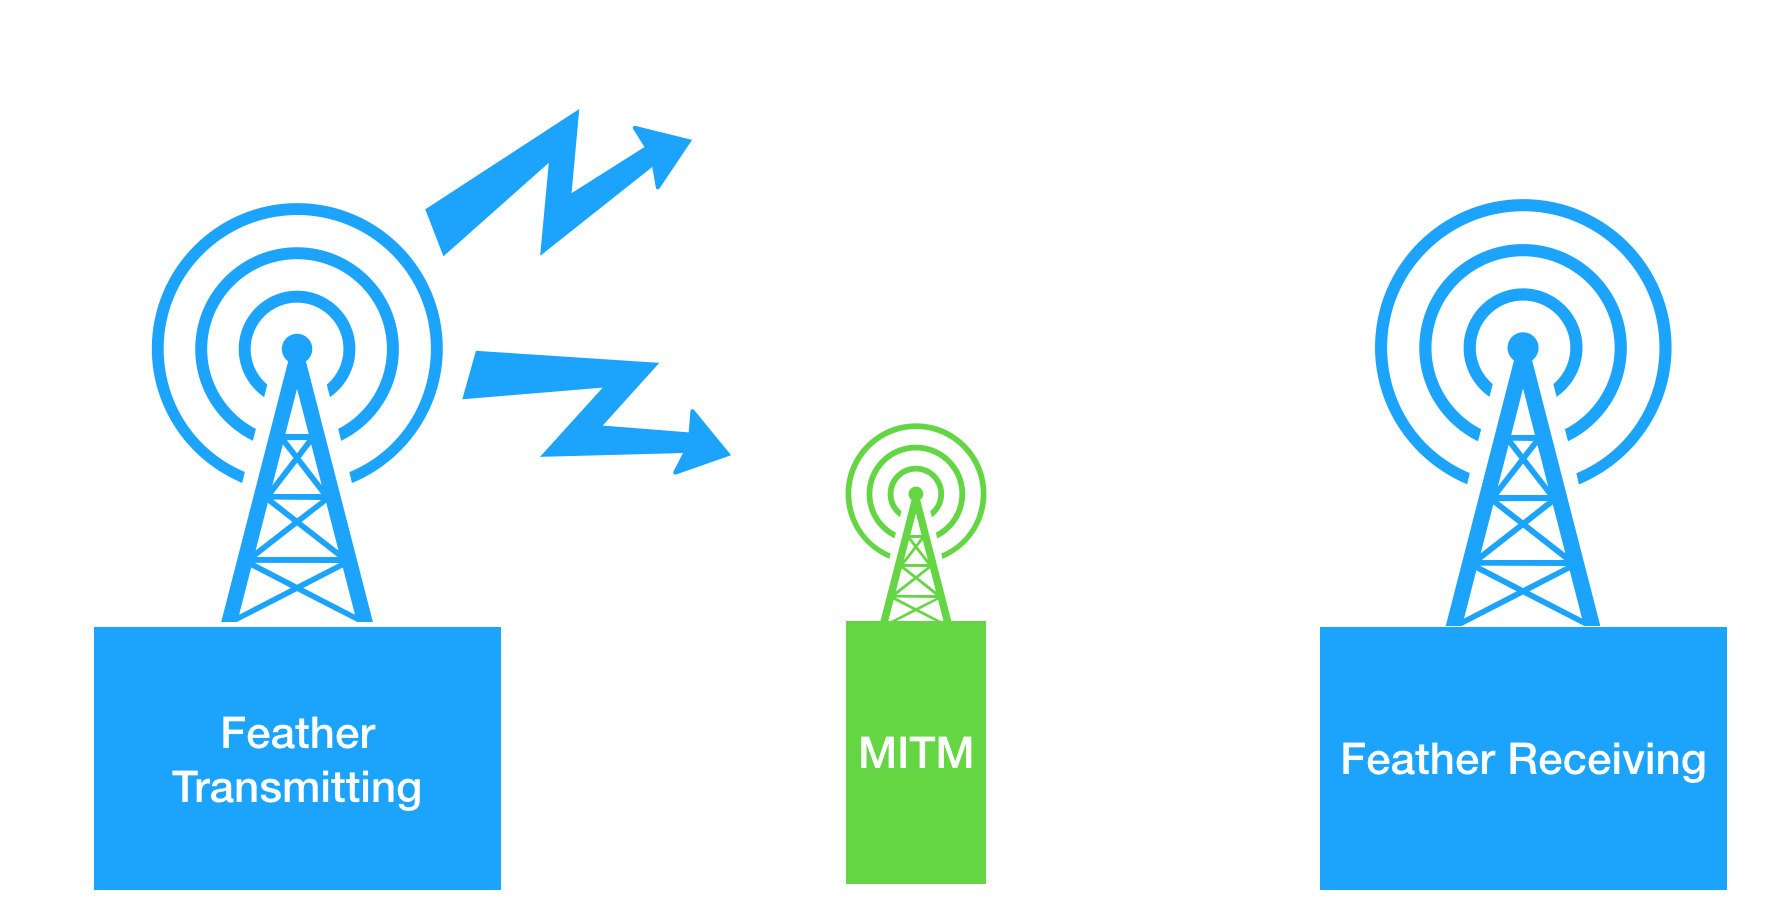
\includegraphics[width=\textwidth]{mitm.png}
\caption{MITM attack on our two feathers}
\label{mitm}
\centrefigureend

In this section we will walk through the steps to looking at the data send over the air.

\centrefigurestart
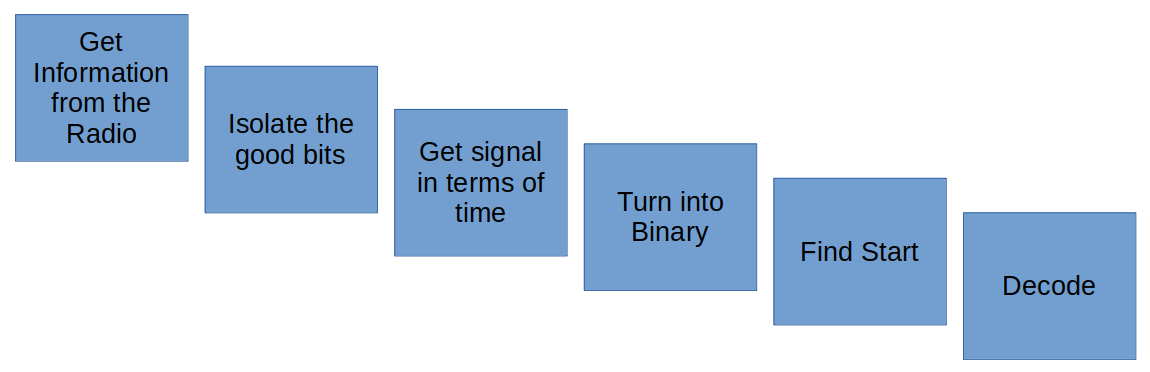
\includegraphics[width=\textwidth]{gnuflow_flow}
\caption{The steps to looking at the data sent}
\label{mitm}
\centrefigureend


\subsection{Connecting the Radio}
In order to get data into the flow from the \gls{sdr} we must use a \gls{source} (just like a river, in gnuradio all data has a source). In this case, it's the RTL-SDR \gls{source} because we are using the RTL-SDR dongle. If there are issues there are plenty of resources available online to work through the RTL-SDR specifics \footnote{\url{https://www.instructables.com/id/RTL-SDR-FM-radio-receiver-with-GNU-Radio-Companion/}}. If you don't have an RTL-SDR the manufacturers website will have documentation of how to use the \gls{sdr} in gnuradio.

\cfbox{blue}{ Find the source in gnuradio using the search button shown in \cref{gnufind}. }

\centrefigurestart

\includegraphics[]{gnuradio_search.png}
\caption{gnuradio-companion search icon}
\label{gnufind}
\centrefigureend

\cfbox{blue}{ Drag in the \gls{source} to the canvas, the canvas should look like the one in \cref{gnusource}. }

\centrefigurestart
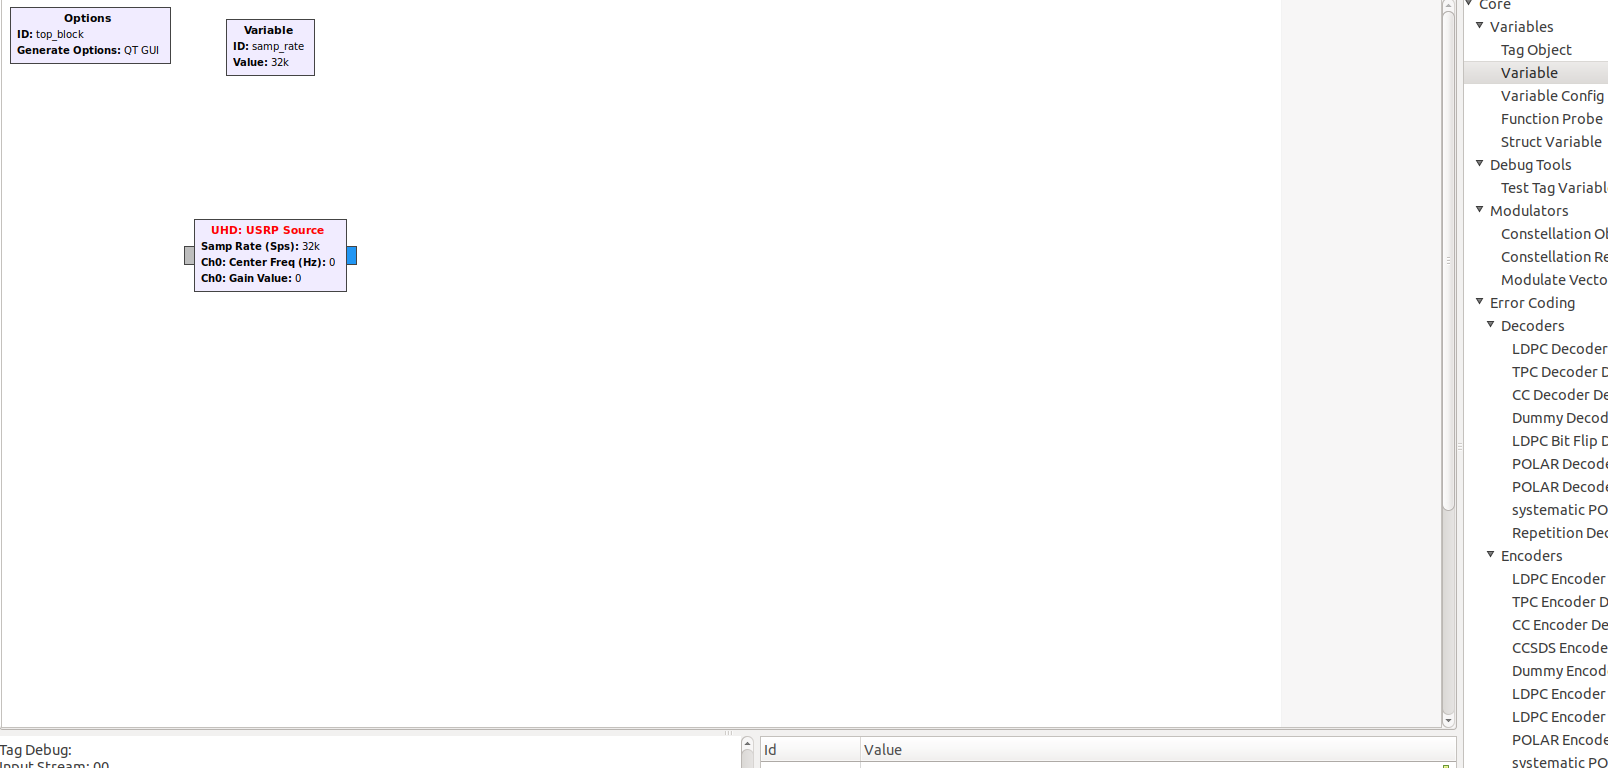
\includegraphics[width=\textwidth]{rtl_src.png}
\caption{A gnuradio flow with just a radio source}
\label{gnusource}
\centrefigureend

\cfbox{blue}{ Double click the \gls{source} block. } 

Here you will get some options, and the key things to find are the \gls{samplerate}, \textit{gain}, and \textit{centre frequency}. The \gls{samplerate} affects how quickly the radio is taking measurements (the rate at which it samples!) and as a result how wide the spectrum we are monitoring is. The gain is how loud that measurement is. The centre frequency is where the middle of the spectrum we are observing sits. The best way for us to experiment with these settings is to use the \textit{QT GUI Range} widget, this widget gives us a slider on the \gls{gui} to change settings at runtime. 

\cfbox{blue}{ Add a QT GUI Range block }

Double click the widget's block and give it a meaningful ID, something like \verb|gain_slider|. Give it a start value of 0, a stop value of 1, and a step of 0.1 as shown in \cref{slider}.

\centrefigurestart
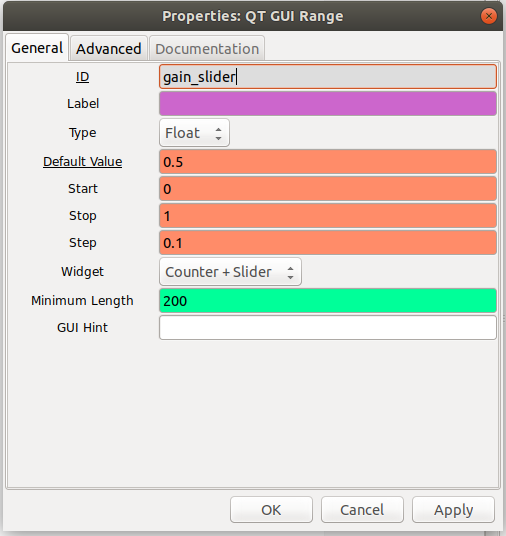
\includegraphics[width=0.5\textwidth]{range_settings}
\caption{Setting up a slider}
\label{slider}
\centrefigureend

Now you can enter it's unique ID in the radio's settings under \textit{gain} as shown in \cref{gain}. This is effectively telling the radio to get it's gain value from the slider called \verb|gain_slider|.

\centrefigurestart
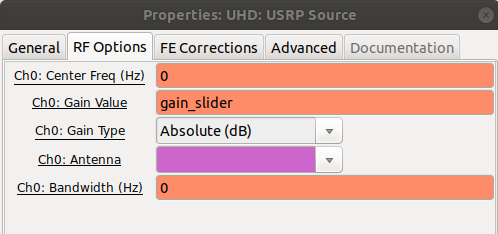
\includegraphics[width=0.5\textwidth]{gain_slider_in_usrp}
\caption{Using a slider value for the gain in the radio source.}
\label{gain}
\centrefigureend


\cfbox{blue}{ Create a slider for the \textit{centre frequency} and \gls{samplerate}. }

Set up your new sliders with the following settings, noting how the \gls{samplerate} is a lot lower than the centre frequency:

\begin{center}
\begin{table}[H]
\begin{tabular}{|c|c|c|c|c|}
\hline
Setting & Start & Stop & Default & Step \\ \hline
Centre Frequency & 430000000 & 440000000 & 435000000 & 500000 \\ \hline
\Gls{samplerate} & 1000000 & 10000000 & 2000000 & 500000 \\ \hline
\end{tabular}
\caption{Radio slider settings}
\end{table}
\end{center}

\subsubsection{Viewing the spectrum}
The next thing is to actually be able to see the spectrum! For this a \textit{QT GUI Frequency Sink} a.k.a. \gls{fftsink} is required. 

\cfbox{blue}{ Add a GT GUI Frequency Sink and connect it shown in \cref{basicflow}. }

Drag this in and connect it to the radio by clicking the blue tabs.

\centrefigurestart
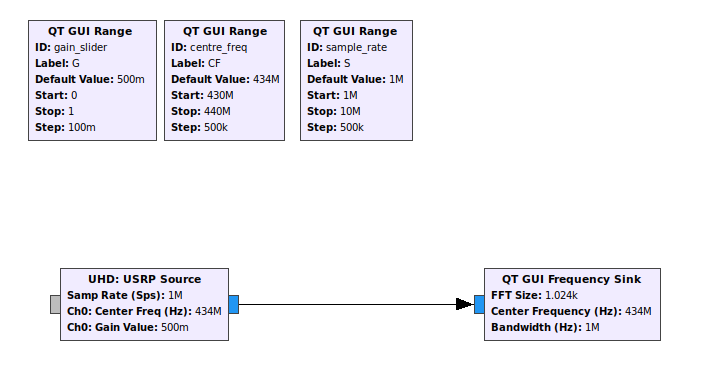
\includegraphics[width=\textwidth]{basic}
\caption{A basic flow.}
\label{basicflow}
\centrefigureend

Again, open the \gls{fftsink} block and set the centre frequency to the same slider as your radio. 

\cfbox{blue}{ Set the bandwidth to your \gls{samplerate} slider as shown in \cref{fftconfig} }

\centrefigurestart
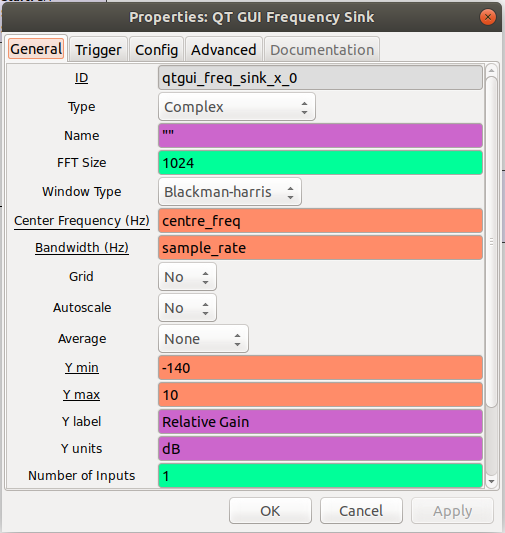
\includegraphics[width=0.5\textwidth]{fft_sink}
\caption{FFT Sink Configuration.}
\label{fftconfig}
\centrefigureend

While you're there, go to the \textit{Config} tab and select \textit{yes} to control panel. 

\cfbox{blue}{ Now, run your flow by clicking the play button at the top of the gnuradio window. }

This will turn your flow into a python script and run it. If there are errors address these before continuing. All being well, the window that pops up should have three sliders, and a very familiar looking spectrum. 

\cfbox{blue}{ Take some time to play with the sliders and see what they do to the spectrum view. (It helps if you enable \textit{max hold} in the spectrum control panel). }

\subsection{Isolating the good bits}

The next step is to use a \gls{lpf} to make sure we receive only the parts of the transmission we are interested in. 

\cfbox{blue}{ Drag an \gls{lpf} into the gnuradio flow, and add another \gls{fftsink} to see the output. }

\cfbox{blue}{ Add some more QT Range Widgets so you can change the parameters of the filter as it's running. }

The parameters of interest here are the \gls{cutoff} (how wide the filter is) and the \gls{transition} (how slopey it's edges are). 

\centrefigurestart
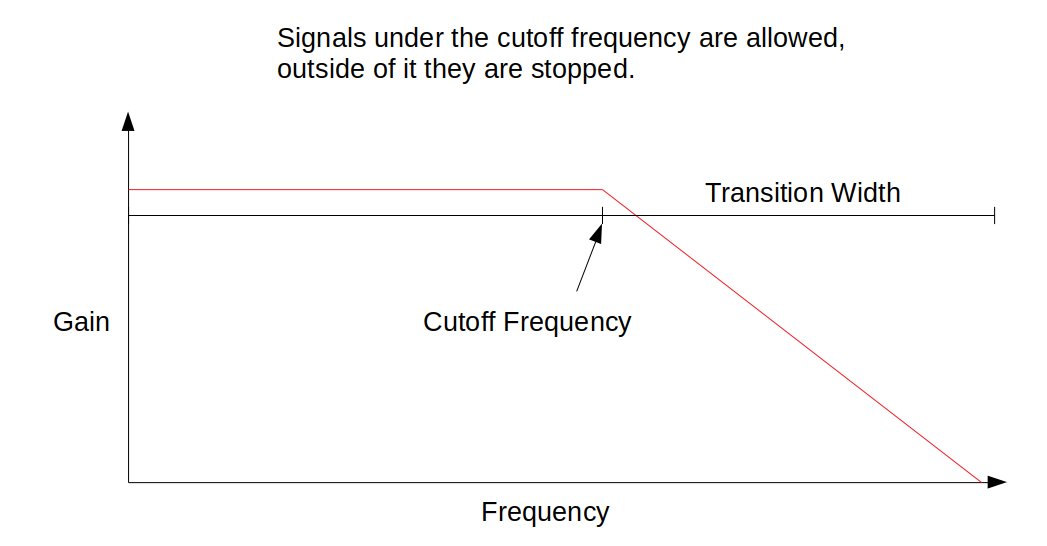
\includegraphics[width=0.5\textwidth]{lpf_filter}
\caption{Where the \gls{cutoff} and \gls{transition}  matter.}
\centrefigureend

Our aim for the \gls{lpf} is to have an output that looks abit like barad-dur.

\begin{figure}[H]
    \centering
    \begin{minipage}{0.45\textwidth}
        \centering
        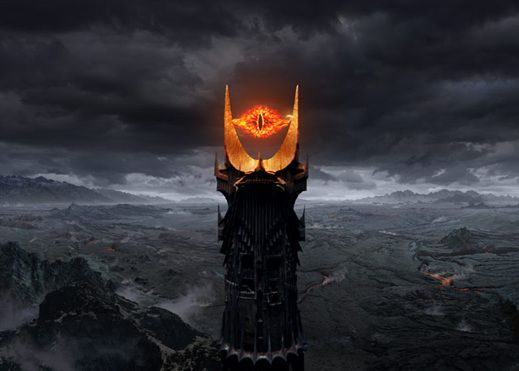
\includegraphics[width=\textwidth]{barad_dur.jpg} 
        \caption{Sauron's home.}
    \end{minipage}\hfill
    \begin{minipage}{0.45\textwidth}
        \centering
        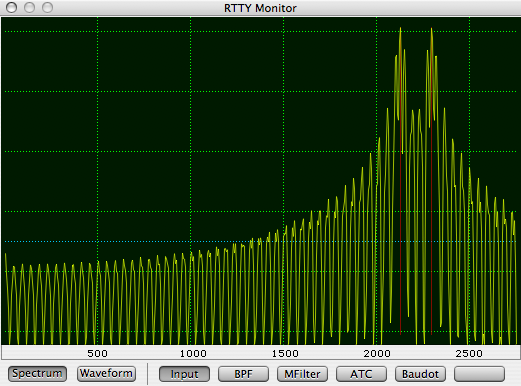
\includegraphics[width=\textwidth]{fsk_plot.png}
        \caption{FSK Signal as seen on a frequency plot.}
    \end{minipage}
\end{figure}

Run your new flow and you should be able to use the filter sliders to isolate specific parts of your signal. I found a value of around 20000 for both to give pretty good results during experimentation. We can further help our filter by using \gls{squelch}. This block will only let signals above a certain amplitude through, effectively cutting out all the noise. 

\cfbox{blue}{ Add a simple \gls{squelch} block after your filter, and set it's \textit{alpha} to 1. }

Again, make a slider for it's \gls{squelch} value and play with it - experiments proved that a value of -40 gave good results for me.

\centrefigurestart
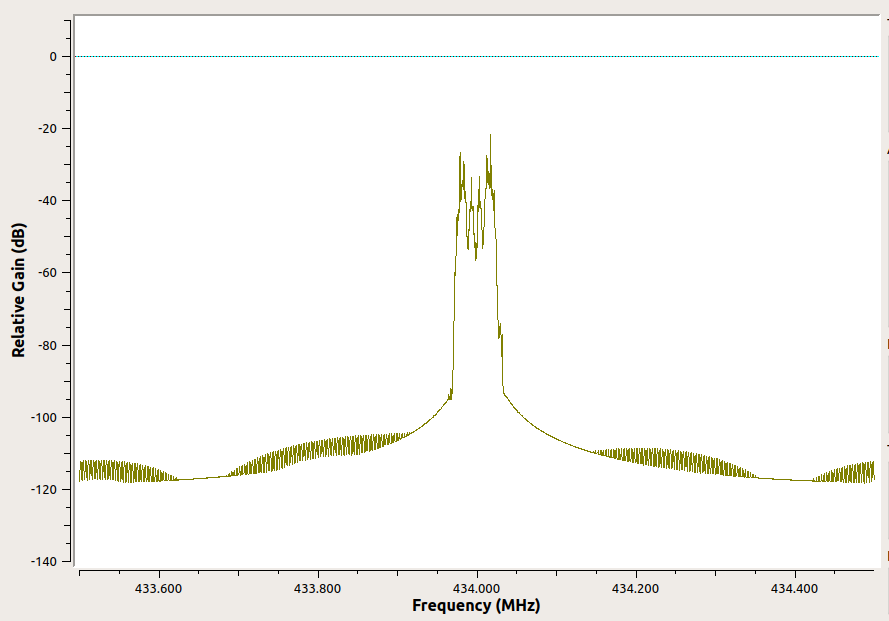
\includegraphics[width=0.5\textwidth]{lpf_peaks}
\caption{An ideal output from the LPF}
\centrefigureend


\centrefigurestart
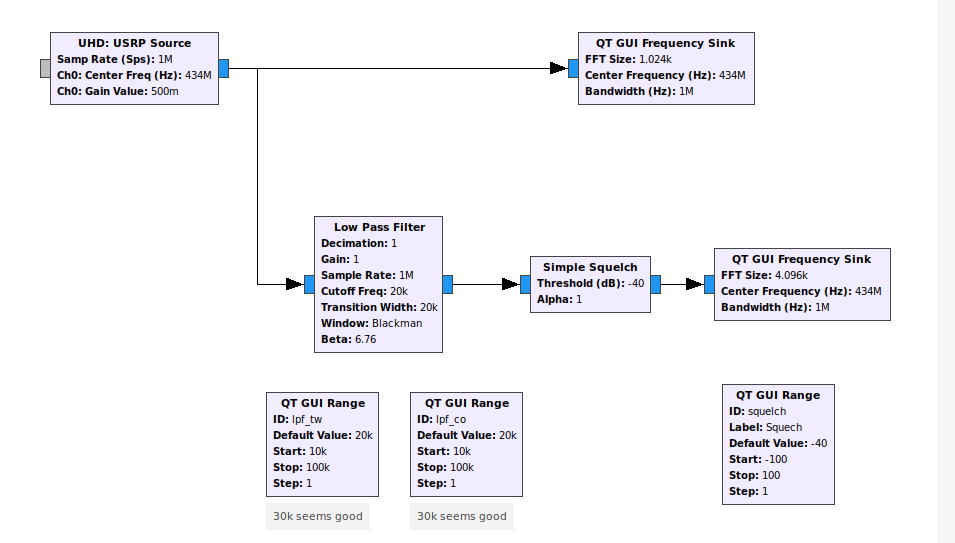
\includegraphics[width=\textwidth]{squelch}
\caption{Radio - LPF - Squelch - Frequency Sink}
\centrefigureend

\subsection{Get signal in terms of time}
Now we have isolated the peaks, we can turn these into bits by using a \Gls{qd} block with a gain setting of 1.

\cfbox{blue}{ Add a \gls{qd} block. }

Plug the output from this into a \textit{QT GUI Time Sink}, and enable the \gls{timesink}'s control panel the same way you did with the \gls{fftsink}. You may have to change the \verb|type| of the the \gls{timesink} in it's config panel so that the blocks join up correctly.

\centrefigurestart
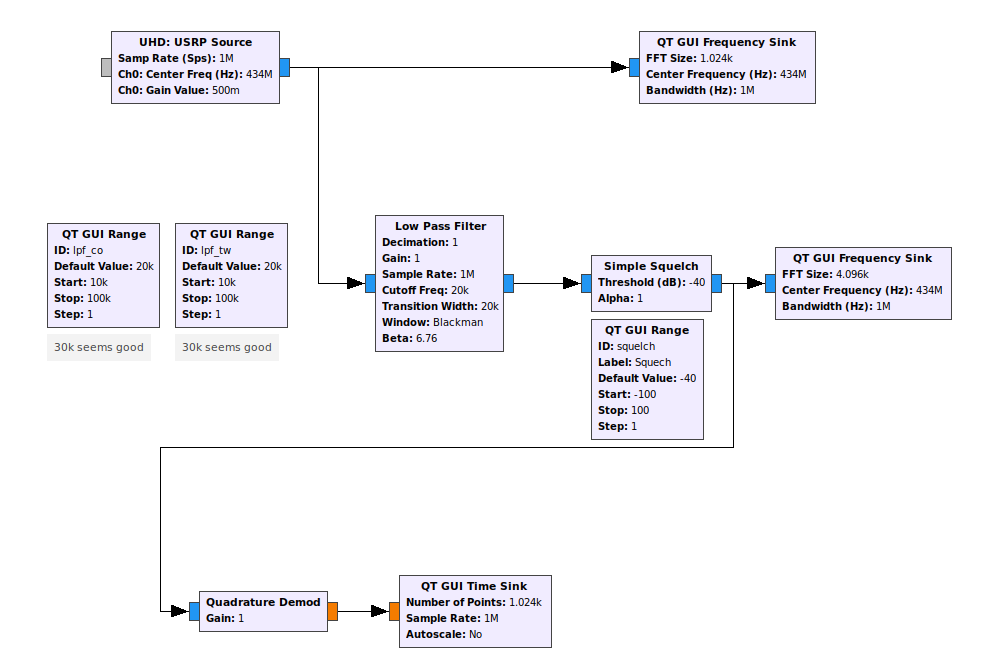
\includegraphics[width=\textwidth]{dq_flow}
\caption{Radio - LPF - Squelch - Quad Demod - Time Sink}
\centrefigureend

This new graph will have turned the frequency changes into changes against time. This will be easier to see in the \gls{timesink} if you set the trigger to auto shown in \cref{auto}, and when the flow is running click '+ X Max' loads until you can see what looks like something interesting like that in \cref{tsoutput}.

\centrefigurestart
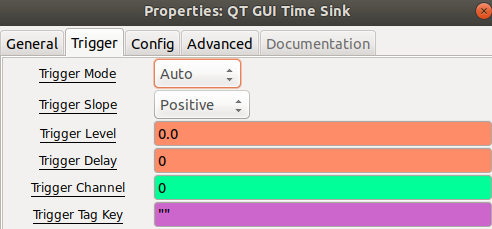
\includegraphics[width=0.5\textwidth]{trig_auto}
\caption{Setting the timesink trigger to auto in the GUI}
\label{auto}
\centrefigureend

\centrefigurestart
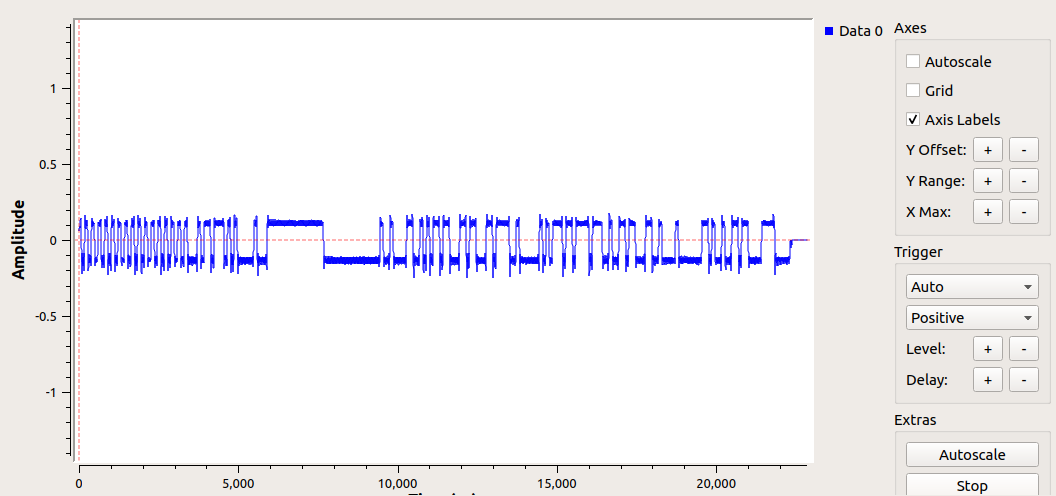
\includegraphics[width=\textwidth]{qd_time}
\caption{Our signal against time}
\label{tsoutput}
\centrefigureend

\subsection{Turn into binary}

In order to turn the signal into binary we need to know exactly when the transition happens. In this section we will do that using the \Gls{crmm} block and a \Gls{binslice}. The \gls{crmm} relies on knowing the \gls{deviation} (how far apart your peaks are in the frequency plot) and your \gls{baudrate} (how quickly bits are sent in the data). Since we made the feathers talk to each other, we know these settings - so it becomes a relatively easy task of plopping numbers into an equation. In the real world however the process of finding this information may take some time and extra snooping around the \gls{RF} spectrum and settings. 

\cfbox{blue}{ Drag in 3 \textit{variable} blocks. } 

Fill the variables with the information in \cref{variablevalues}.

\begin{table}[H]
\begin{tabular}{|c|c|}
\hline
Variable Name & Value \\ \hline
baudrate\_hz & 9600 \\ \hline
deviation\_hz & 19200 \\ \hline
samples\_per\_symbol & sample\_rate/baudrate\_hz \\ \hline
\end{tabular}
\caption{Variable values}
\label{variablevalues}
\end{table}

\cfbox{blue}{ Add a \Gls{crmm} block. }

Then, in your clock recovery block set the \textit{omega} to be \verb|samples_per_symbol| like in \cref{crconfig}

\centrefigurestart
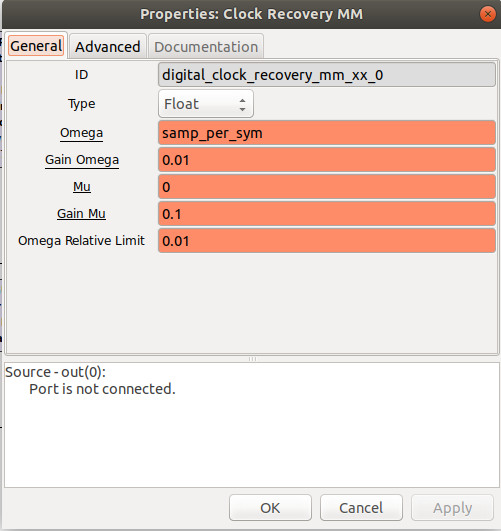
\includegraphics[width=0.5\textwidth]{clock_recovery}
\caption{Clock recovery block settings}
\label{crconfig}
\centrefigureend

\cfbox{blue}{ Connect a \gls{timesink} to this to see the output. }

\centrefigurestart
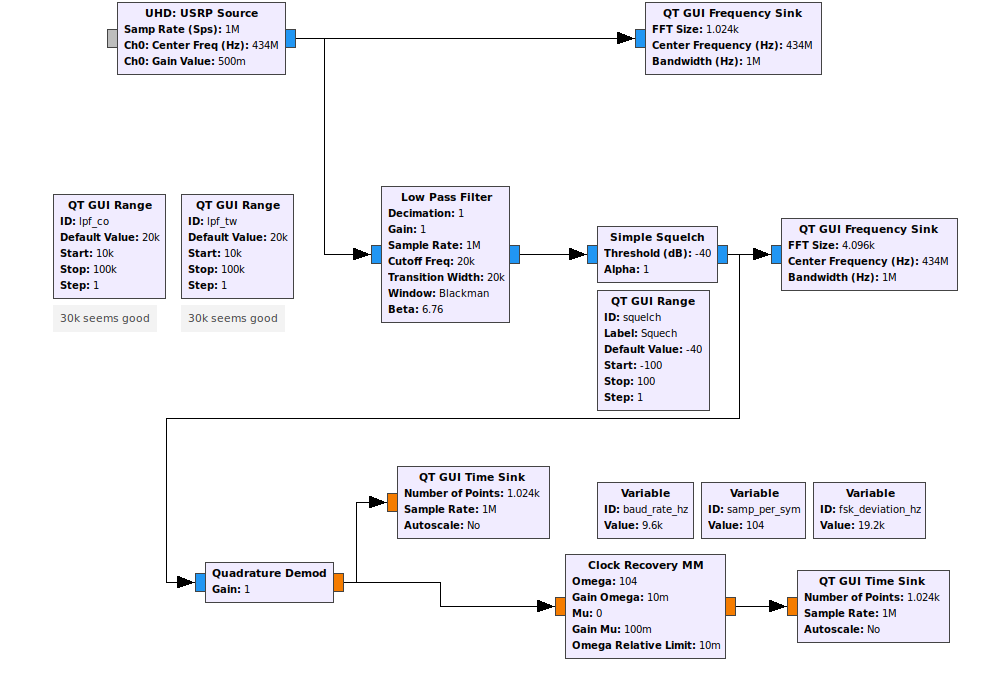
\includegraphics[width=\textwidth]{clk_recovery_flow}
\caption{Radio - Filter - Squelch - Quad Demod - Clock Recovery}
\centrefigureend

What you should see is a slight difference between the \gls{timesink}s for just the \gls{qd} and the \gls{crmm}. The \gls{crmm} one will look a bit pointier, and the lines will be less thick. This is clearest at the start of the graph - one data point will be high, and the next low whereas without the \gls{crmm} this part of this signal has 'fatter' highs and lows. A comparison can be seen in \cref{binslice} and \cref{bindetail}.

\centrefigurestart
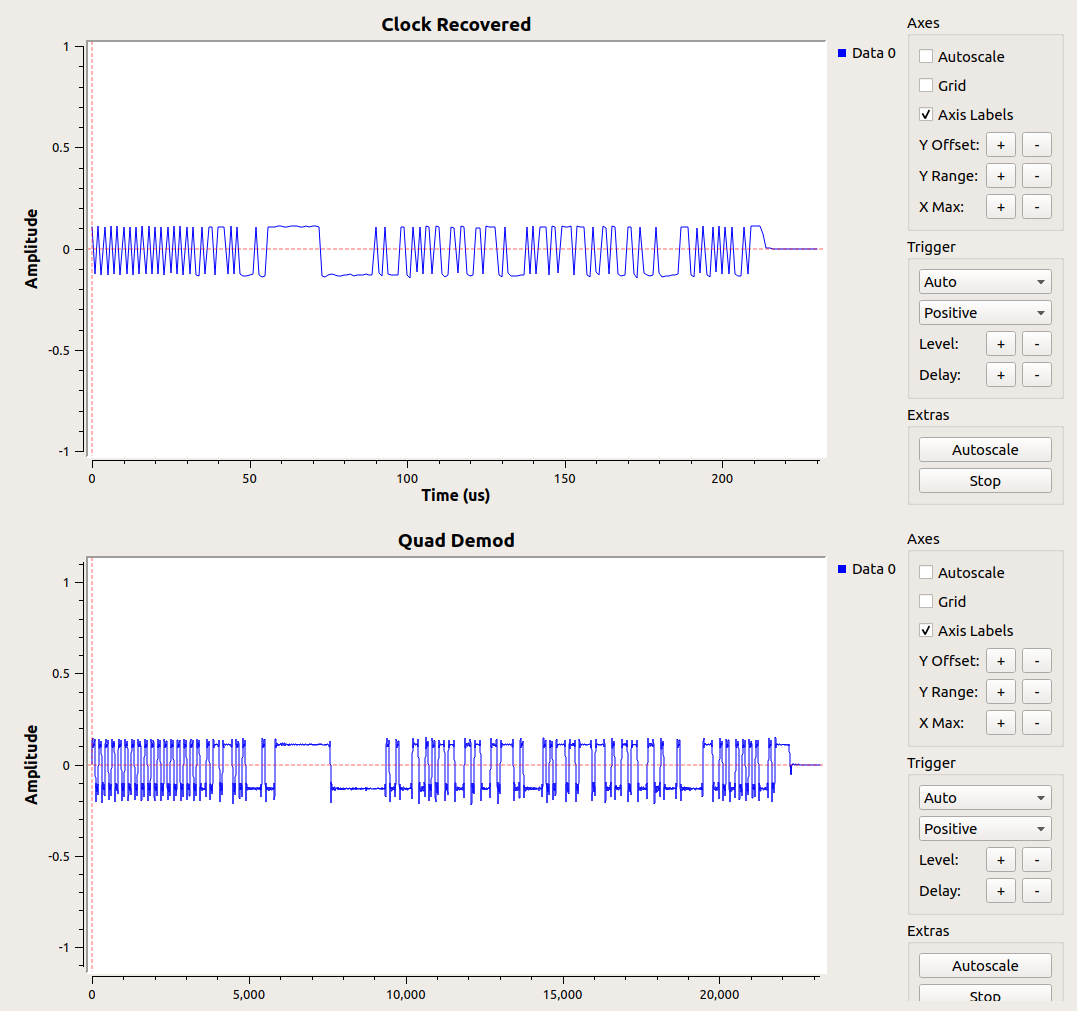
\includegraphics[width=\textwidth]{clock_vs_qd_time}
\caption{The signal before and after clock recovery}
\label{binslice}
\centrefigureend

\centrefigurestart
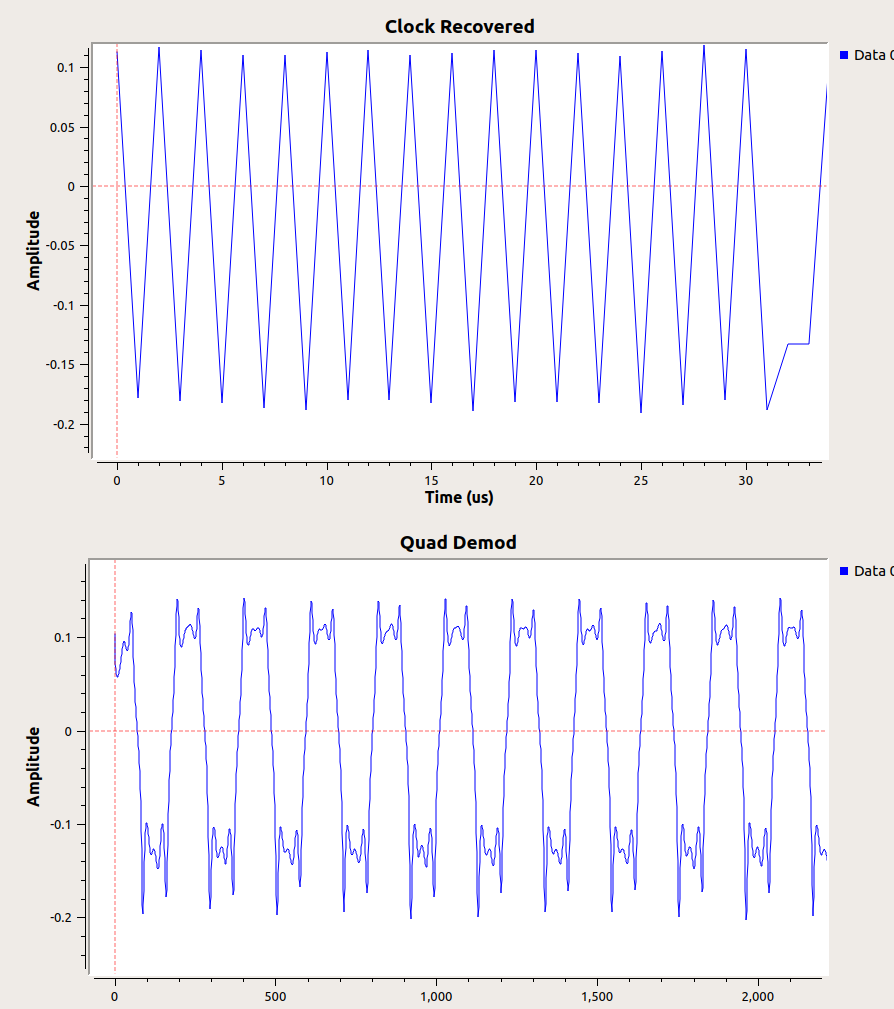
\includegraphics[width=\textwidth]{clk_recovery_vs_qd_zoom}
\caption{Detail of a series of 1 and 0 before and after clock recovery}
\label{bindetail}
\centrefigureend

\cfbox{blue}{ Finally add a \textit{binary slicer} to the end of the clock recovery block. }

Done.

\subsection{Find start}
Finding the start of the signal is relatively easy as a block called \Gls{cac} will do this by searching for a pattern in the binary stream coming in. Through inspection of the \gls{timesink}s before we can see that the signal starts with a long stream of 1 and 0. This is known as the \gls{preamble} and is present in lots of signals; it's the radio's way of saying 'LISTEN TO ME I'M TRANSMITTING' before it sends any useful data. In your new block set the \verb|Access Code| to be 1010101010101010101010101010101000101101 (or 4 bytes of 10101010 then a byte of 00101101), a threshold of 0, and call the tag \verb|preamble|.

\centrefigurestart
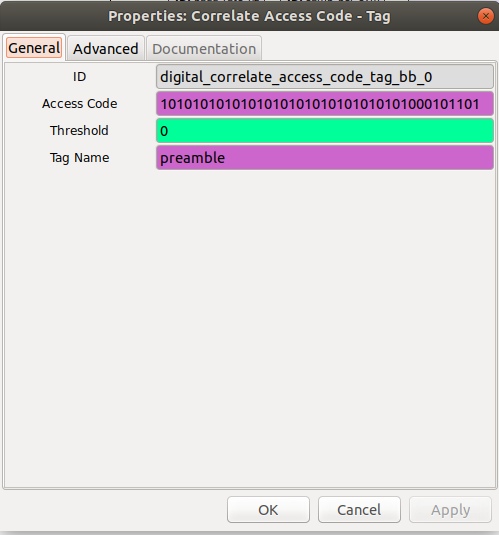
\includegraphics[width=0.5\textwidth]{cac_settings}
\caption{Correlate Access Code Settings}
\centrefigureend

This block, when it sees a stream of data matching the access code will insert a special tag into the data stream with the name 'preamble' to show that it's detected a \gls{preamble}. Finally output this to a file using a \textit{File Meta \Gls{sink}}. This file may grow quite large so I recommend making something like \verb|tmp/file_sink| so that it's deleted when you turn off your computer.

\centrefigurestart
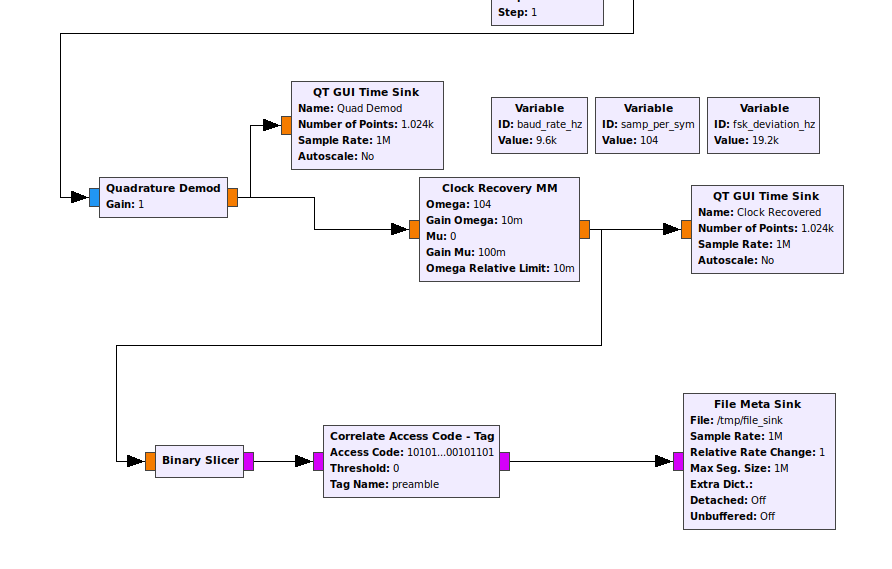
\includegraphics[width=\textwidth]{full_Flow}
\caption{Radio - LPF - Squelch - Quad Demod - Clock Recovery - Binary Slicer - Correlate Access Code - File Sink}
\centrefigureend
\subsection{Decode}
This is where it can get abit tougher! I have cobbled together a small tool to help. It's not that great and misses some of the messages, however it's a start! In the \gls{repo} you downloaded use the analyser to examine the contents of the file you created. This tool looks for the 'preamble' tag in the file and then prints off a certain number of bytes afterwards to the screen. In order to build the tool navigate to it's directory and enter the command \verb|source doit.sh|. This will create a folder called \verb|build| and make the application there. Then you can use it by entering the command \verb|./analyser /tmp/file_sink| and it should print off some of the packets.

\centrefigurestart
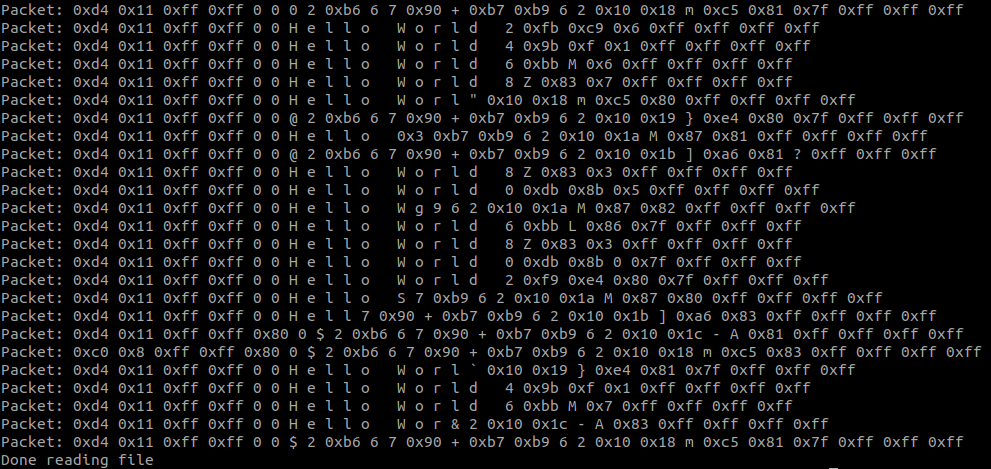
\includegraphics[width=\textwidth]{packets}
\caption{Output of the analyser}
\centrefigureend

It appears to skip every other packet at this stage however we can clearly see a bunch of 'Hello World' messages decoded - congratulations you have successfully performed a \gls{mitm} attack on your feather!

A full flow is available to do this in the \gls{repo} - if you get stuck at any point.
